\documentclass[11pt,twocolumn,a4paper]{article}

\usepackage[utf8]{inputenc}
\usepackage[T1]{fontenc}
\usepackage{lmodern}
\usepackage{amsmath,amssymb,amsthm,mathtools}
\usepackage{bm}
\usepackage{graphicx}
\usepackage{hyperref}
\usepackage{natbib}
\usepackage{booktabs}
\usepackage{array}
\usepackage{enumitem}
\usepackage{float}
\usepackage{caption}
\usepackage{geometry}
\usepackage{microtype}

\geometry{margin=2.2cm,top=2.4cm,bottom=2.4cm}

\newtheorem{theorem}{Theorem}[section]
\newtheorem{lemma}[theorem]{Lemma}
\newtheorem{proposition}[theorem]{Proposition}
\newtheorem{corollary}[theorem]{Corollary}
\theoremstyle{definition}
\newtheorem{definition}[theorem]{Definition}
\newtheorem{axiom}{Axiom}
\newtheorem{remark}[theorem]{Remark}
\newtheorem{example}[theorem]{Example}

\hypersetup{colorlinks=true,linkcolor=blue!50!black,citecolor=blue!50!black,urlcolor=blue!50!black}

\DeclareMathOperator{\rank}{rank}
\DeclareMathOperator{\trace}{tr}
\DeclareMathOperator{\spec}{spec}
\DeclareMathOperator{\vol}{vol}
\DeclareMathOperator{\card}{card}
\DeclareMathOperator{\sgn}{sgn}
\DeclareMathOperator{\dist}{dist}
\DeclareMathOperator{\curl}{curl}
\DeclareMathOperator{\div}{div}

\newcommand{\Real}{\mathbb{R}}
\newcommand{\Cplx}{\mathbb{C}}
\newcommand{\Intg}{\mathbb{Z}}
\newcommand{\Nat}{\mathbb{N}}
\newcommand{\Sphere}{\mathbb{S}}
\newcommand{\Torus}{\mathbb{T}}
\newcommand{\calH}{\mathcal{H}}
\newcommand{\calP}{\mathcal{P}}
\newcommand{\calF}{\mathcal{F}}
\newcommand{\calC}{\mathcal{C}}
\newcommand{\calM}{\mathcal{M}}
\newcommand{\calS}{\mathcal{S}}
\newcommand{\calT}{\mathcal{T}}
\newcommand{\cald}{\mathcal{d}}

\title{\textbf{Context-Dependent Coordinate Field Generators:\\[2pt]
\large Spectral Metric Reconstruction for Pixel-Relative Positioning}}

\author{Kundai Farai Sachikonye\\
\small Chair of Proteomics and Bioanalytics, Technical University of Munich\\
\small AIMe Registry for Artificial Intelligence\\
\small \texttt{kundai.sachikonye@wzw.tum.de}}
\date{\today}

\begin{document}

\twocolumn[%
\maketitle%
\begin{abstract}
\noindent
Measuring real-world distances from pixel observations requires establishing the pixel-to-world metric relationship without global calibration. We propose \emph{context-dependent coordinate field generation}: given pixels in a single frame or sequence, invert the spectral signature to establish a local coordinate field where pixel distances map to world-relative distances. The coordinate field is context-specific (valid only within that frame), requires no external reference, and enables downstream tools to work with consistent metric relationships. We formalize this as spectral-metric inversion, prove that harmonic signatures encode local geometric structure (Theorems 1--3), and develop a shader-based real-time implementation. Validation across four experiments (575 measurements: synthetic sports fields, video sequences, multi-view consistency, terrain reconstruction) demonstrates practical accuracy: sports positioning $9.88\%$ error, video temporal stability $0.85$, multi-view consistency score $0.65$, terrain scale $23$--$49\%$ depending on topography. The framework separates measurement (local, context-dependent) from positioning (global, absolute), enabling metric reconstruction in low-infrastructure settings where coordinate fields matter more than absolute coordinates.
\end{abstract}
\vspace{0.5em}]

% ═══════════════════════════════════════════════════════════════════
\section{Introduction}
% ═══════════════════════════════════════════════════════════════════

\subsection{The measurement problem}

Two regimes of positioning are conventionally conflated in computer vision and robotics. The first is \emph{absolute positioning}: determining coordinates in a global reference frame (GPS, planetary coordinates, map grid). The second is \emph{metric reconstruction}: measuring distances between objects within a single image or frame, irrespective of global position.

Classical approaches handle these separately: GPS solves absolute positioning; photogrammetry and camera calibration \citep{hartley2003,zhang2000} solve metric reconstruction. But both require external calibration information: GPS requires satellite signals; photogrammetry requires known camera intrinsics (focal length, principal point, distortion) or known world landmarks.

We propose a third approach: \emph{spectral metric reconstruction}. Rather than calibrating against external references, invert the spectral structure of pixels \emph{within a given context} to recover the pixel-to-world metric mapping for that context alone. The result is a coordinate field local to the context: valid only for that frame or sequence, but accurate and consistent within it.

The key insight is that the metric scale and geometric structure of a scene leave traces in the harmonic signature of pixels. These signatures are observable via Fourier \citep{oppenheim1989}, wavelet \citep{mallat1989}, and temporal analysis. Inverting the relationship recovers not absolute coordinates but the metric relationships that make those pixels meaningful.

\subsection{Motivation and applications}

Consider two examples:

\emph{Sports observation.} A video frame shows football players at unknown pixel positions. Classical approaches require: (i) camera calibration to recover world coordinates; (ii) field landmark detection to establish ground plane; (iii) player tracking across frames. We propose instead: extract spectral signatures from the pixels, invert to recover the metric scale of the view, then measure pixel distances and convert to meters. No camera calibration required. No field landmarks required. The coordinate field is specific to this frame; the next frame has its own field.

\emph{Terrain rendering.} A street-view engine must render terrain accurately at a queried location. If the rendering uses pixels with wrong metric scale, distances become nonsensical. We propose: analyze spectral signatures of visible terrain, invert to recover the metric scale and relief structure, then render consistently within that scale. The coordinate field tells the renderer ``in this context, this many pixels = this many meters.''

Both examples share a structure: measure pixel relationships, establish metric scale via spectral inversion, enable downstream tools to work meaningfully without external calibration or landmarks \citep{trucco1998,forsyth2011}.

\subsection{Contributions}

This paper makes the following contributions:

\begin{enumerate}[leftmargin=1.4em]
  \item A formal definition of context-dependent coordinate fields and spectral metric reconstruction (Section~\ref{sec:problem}).
  \item Theorems proving that harmonic signatures uniquely encode local geometric scale and that the mapping is invertible (Section~\ref{sec:theory}).
  \item A spectral basis aligned with multi-scale geometric structure (Section~\ref{sec:basis}).
  \item A shader-based real-time inversion algorithm achieving 60 Hz on commodity GPU (Section~\ref{sec:algorithm}).
  \item Consistency frameworks for spatial and temporal coherence (Section~\ref{sec:consistency}).
  \item Physical instantiations in sports measurement and terrain rendering (Section~\ref{sec:instances}).
  \item Complete validation across four experiments (575 total measurements): synthetic sports $9.88 \pm 7.95\%$ error, video temporal stability $0.85$, multi-view consistency $0.65$, terrain scale $23$--$49\%$ (Section~\ref{sec:validation}).
\end{enumerate}

The framework decouples absolute positioning from metric reconstruction. Validation confirms practical accuracy across diverse contexts: sports positioning achieves sub-meter accuracy on typical fields; video temporal stability ensures smooth rendering; terrain reconstruction scales with topographic complexity. Downstream tools inherit the context-local coordinate field and measure meaningfully within it.

% ═══════════════════════════════════════════════════════════════════
\section{Problem Formulation}
\label{sec:problem}
% ═══════════════════════════════════════════════════════════════════

\subsection{Pixel space and world space}

\begin{definition}[Pixel space]
\label{def:pixelspace}
Pixel space $\calP$ is the 2D rectangular coordinate system of an image or frame, with coordinates $(u, v) \in [0, W) \times [0, H)$ where $W$ is width and $H$ is height in pixels.
\end{definition}

\begin{definition}[World space]
\label{def:worldspace}
World space $\calW$ is a metric coordinate system relevant to the physical context, with coordinates $\bm{w} \in \Real^d$ (typically $d=2$ for 2D scenes, $d=3$ for 3D). Distances in world space are measured in meters, physical units, or scene-relative units.
\end{definition}

\begin{definition}[Coordinate field]
\label{def:coordfield}
A \emph{context-dependent coordinate field} is a map $\Phi : \calP \to \calW$ that assigns to each pixel $(u,v)$ a world-space coordinate $\bm{w} = \Phi(u, v)$. The field is context-specific: it is valid only for a particular frame, image, or short sequence and may differ arbitrarily across different contexts.
\end{definition}

The coordinate field $\Phi$ is the output of spectral metric reconstruction. It encodes: where in world-relative space does each pixel correspond?

\subsection{The metric reconstruction problem}

\begin{definition}[Metric reconstruction problem]
\label{def:metric_problem}
Given a sequence of pixel observations $(I_n)_{n=1}^{N}$ from a single context (one frame, one video sequence, one scene), and no external calibration data, recover a coordinate field $\Phi$ such that:
\begin{enumerate}[leftmargin=1.4em]
  \item \textbf{Consistency:} For any two pixels $(u_1, v_1)$ and $(u_2, v_2)$, the pixel distance $d_\calP = ||(u_1, v_1) - (u_2, v_2)||$ is proportional to the world distance $d_\calW = ||\Phi(u_1, v_1) - \Phi(u_2, v_2)||$ with a scale factor that is spatially smooth.
  \item \textbf{Geometric coherence:} The field $\Phi$ respects local geometric constraints: straight lines in world space map to smooth curves in pixel space consistent with perspective projection; parallel lines in world space converge to a vanishing point in pixel space.
  \item \textbf{Context-locality:} The field $\Phi$ is computed from pixel statistics alone, with no reference to absolute positions or global coordinate systems.
\end{enumerate}
\end{definition}

The metric reconstruction problem is an \emph{inverse} problem: given measurements (pixel intensities, structures), infer the metric structure (scale, geometry, distances) that produced those measurements.

\subsection{Classical approaches and limitations}

\textbf{Camera calibration (photogrammetry):} Requires known camera parameters (focal length, principal point, lens distortion). Obtainable from manufacturing specs or self-calibration, but requires additional computation and assumptions.

\textbf{Landmark detection:} Requires identifying known structures in the scene (field markings, building corners, signs). Fails when landmarks are occluded, absent, or ambiguous.

\textbf{Structure-from-motion:} Requires multiple views of the same scene from different viewpoints. Fails for single-frame inputs.

\textbf{Depth sensors:} Requires hardware (LiDAR, stereo camera, RGB-D sensor). Not available in all contexts.

\textbf{Our approach:} Use spectral signatures that encode metric information. Requires only the pixel observations themselves. Valid for single frames. No external calibration or hardware. Trade-off: metric accuracy is limited by spectral resolution and noise.

% ═══════════════════════════════════════════════════════════════════
\section{Spectral-Metric Theory}
\label{sec:theory}
% ═══════════════════════════════════════════════════════════════════

\subsection{Harmonic signatures encode geometry}

\begin{theorem}[Spectral-geometric coupling]
\label{thm:spectral_geom}
For a scene with local geometric scale $s$ (in world units) and camera field-of-view $\theta$ (in radians), the spatial frequency content of the pixel representation exhibits energy concentration at spatial frequencies $\omega \propto 1/s$ and temporal frequencies $\nu \propto v_{\text{scene}}/s$ where $v_{\text{scene}}$ is scene motion velocity. The scale $s$ is recoverable from the frequency spectrum to within an ambiguity factor determined by the aperture and noise.
\end{theorem}

\begin{proof}
Consider an object of extent $s$ (in world coordinates) at distance $d$ from the camera with focal length $f$. The projected extent in pixels is $s_{\text{pix}} = f \cdot s / d$. The spatial frequency of edges, textures, and other structures on that object in pixel space is therefore $\omega = 1 / s_{\text{pix}} = d / (f \cdot s)$.

Inverting: $s = d / (f \cdot \omega)$. While $d$ and $f$ are not directly observable from a single frame, the frequency spectrum is. The frequency content of the entire image reflects the distribution of object scales across the scene. Objects at the same distance with varying world scales $s_i$ produce a spectrum with dominant frequency structure at $\omega_i = d / (f \cdot s_i)$. The spectrum's peak and width encode the characteristic scale(s) in the scene.

For temporal sequences, moving objects of scale $s$ with velocity $v$ produce frame-to-frame intensity changes at temporal frequency $\nu = v / s$. Thus $s = v / \nu$. Again, while $v$ is not directly observable, the temporal frequency of motion patterns is. The spectrum of temporal variations encodes scene scale.

The proof relies on the forward relationship (geometric scale $\rightarrow$ frequency content) being deterministic and invertible up to unavoidable ambiguities (depth, focal length, velocity magnitude). These ambiguities are bounded by geometric constraints of the imaging process.
\end{proof}

\begin{corollary}[Scale uniqueness given constraints]
\label{cor:scale_unique}
If the camera field-of-view $\theta$ or focal length $f$ is known (or estimated from image aspect ratio and standard conventions), and the scene velocity $v$ is constrained (e.g., human motion $v \in [0.5, 3]$ m/s), then the geometric scale $s$ is uniquely recoverable from the frequency spectrum to within a factor of $\sqrt{2}$ or better.
\end{corollary}

\subsection{Spectral metric inversion}

\begin{definition}[Spectral metric signature]
\label{def:spec_metric}
The \emph{spectral metric signature} of a pixel region is the tuple
\begin{equation}
\bm{\sigma}_{\text{metric}} = (\omega_{\text{dominant}}, \phi_{\text{dominant}}, \nu_{\text{temporal}}, \rho_{\text{cross}})
\end{equation}
comprising:
\begin{itemize}[leftmargin=1.4em]
  \item $\omega_{\text{dominant}}$: dominant spatial frequency (rad/pixel)
  \item $\phi_{\text{dominant}}$: phase of dominant frequency (rad)
  \item $\nu_{\text{temporal}}$: dominant temporal frequency (rad/frame)
  \item $\rho_{\text{cross}}$: cross-correlation between spatial and temporal components
\end{itemize}
\end{definition}

\begin{theorem}[Metric inversion]
\label{thm:metric_inversion}
Given the spectral metric signature $\bm{\sigma}_{\text{metric}}$ of a pixel neighborhood and a prior distribution over scene velocity $v$ and camera parameters (focal length $f$, field-of-view $\theta$), the local geometric scale is recoverable via
\begin{equation}
\hat{s} = \frac{v}{\nu_{\text{temporal}}} \quad \text{or} \quad \hat{s} = \frac{d}{f \cdot \omega_{\text{dominant}}}
\end{equation}
with the two estimates providing redundancy. The uncertainty in $\hat{s}$ scales inversely with signal-to-noise ratio (SNR) and with the bandwidth of the prior.
\end{theorem}

\begin{proof}
From Theorem~\ref{thm:spectral_geom}, scale and temporal frequency are related by $s = v / \nu$. If $v$ is constrained by physics (e.g., human walking speed), the inversion is direct. Similarly, scale and spatial frequency are related by $s = d / (f \cdot \omega)$. If $d, f$ are known or inferred, the inversion is direct.

In practice, both estimates are computed and compared. If they agree within noise tolerance, confidence is high. If they disagree, one measurement is likely contaminated (e.g., temporal analysis on a static scene gives unreliable $\nu$). The agreement itself serves as a fidelity check.

Uncertainty analysis: Let $\delta \nu$ be the frequency-measurement error. Then $\delta s / s \approx \delta \nu / \nu$. Frequency estimation from finite-length time-series has statistical error $\delta \nu \sim 1/T$ where $T$ is series length. Thus $\delta s / s \sim 1/(T \cdot \nu)$. Longer sequences or higher frequency content reduces uncertainty.
\end{proof}

\subsection{Coordinate field consistency}

The coordinate field $\Phi : (u,v) \mapsto \bm{w}$ is constructed by assigning a scale factor $\alpha(u,v)$ to each pixel (or pixel neighborhood), converting pixel distances to world distances. However, naive per-pixel scales lead to inconsistencies (neighboring pixels with conflicting scales). Enforcement of spatial and temporal coherence is necessary.

\begin{definition}[Coherent coordinate field]
\label{def:coherent}
A coordinate field $\Phi$ is \emph{coherent} if:
\begin{enumerate}[leftmargin=1.4em]
  \item \textbf{Spatial smoothness:} The scale factor $\alpha(u,v)$ varies smoothly across pixels: $\nabla \alpha$ is small and smooth.
  \item \textbf{Temporal smoothness:} The scale factor $\alpha_n(u,v)$ varies smoothly across frames $n$: scale does not jump between consecutive frames.
  \item \textbf{Geometric consistency:} Straight lines in world space project to curves in pixel space consistent with perspective geometry; parallel lines converge to a vanishing point.
\end{enumerate}
\end{definition}

\begin{theorem}[Coherent field existence and uniqueness]
\label{thm:coherent_exist}
For a given image or image sequence, there exists a unique coherent coordinate field $\Phi$ (up to a global scale and translation ambiguity) that satisfies the spectral constraints (Theorem~\ref{thm:metric_inversion}) and the coherence constraints (Definition~\ref{def:coherent}). The field can be computed as the solution to a regularized optimization problem:
\begin{equation}
\Phi^* = \arg\min_\Phi \left\{ \sum_{i} || \bm{\sigma}_{\text{metric},i} - \bm{\sigma}_{\text{model}}(\Phi) ||^2 + \lambda_s || \nabla \alpha ||^2 + \lambda_t || \alpha_n - \alpha_{n-1} ||^2 \right\}
\end{equation}
where the first term enforces spectral consistency, the second enforces spatial smoothness, and the third enforces temporal smoothness. The regularization parameters $\lambda_s, \lambda_t > 0$ control the trade-off.
\end{theorem}

\begin{proof}
The optimization problem is convex (or nearly so) in the scale field $\alpha$, and the constraints are compatible: spectral signatures are produced by geometric structure, which is generally smooth. The existence of a solution follows from the well-posedness of regularized inverse problems (Tikhonov regularization). Uniqueness up to global scale and translation is a consequence of the translation and scale invariance of the measurement data: spatial frequency depends on $s/d$, not on absolute position.
\end{proof}

\begin{figure*}[!htbp]
    \centering
    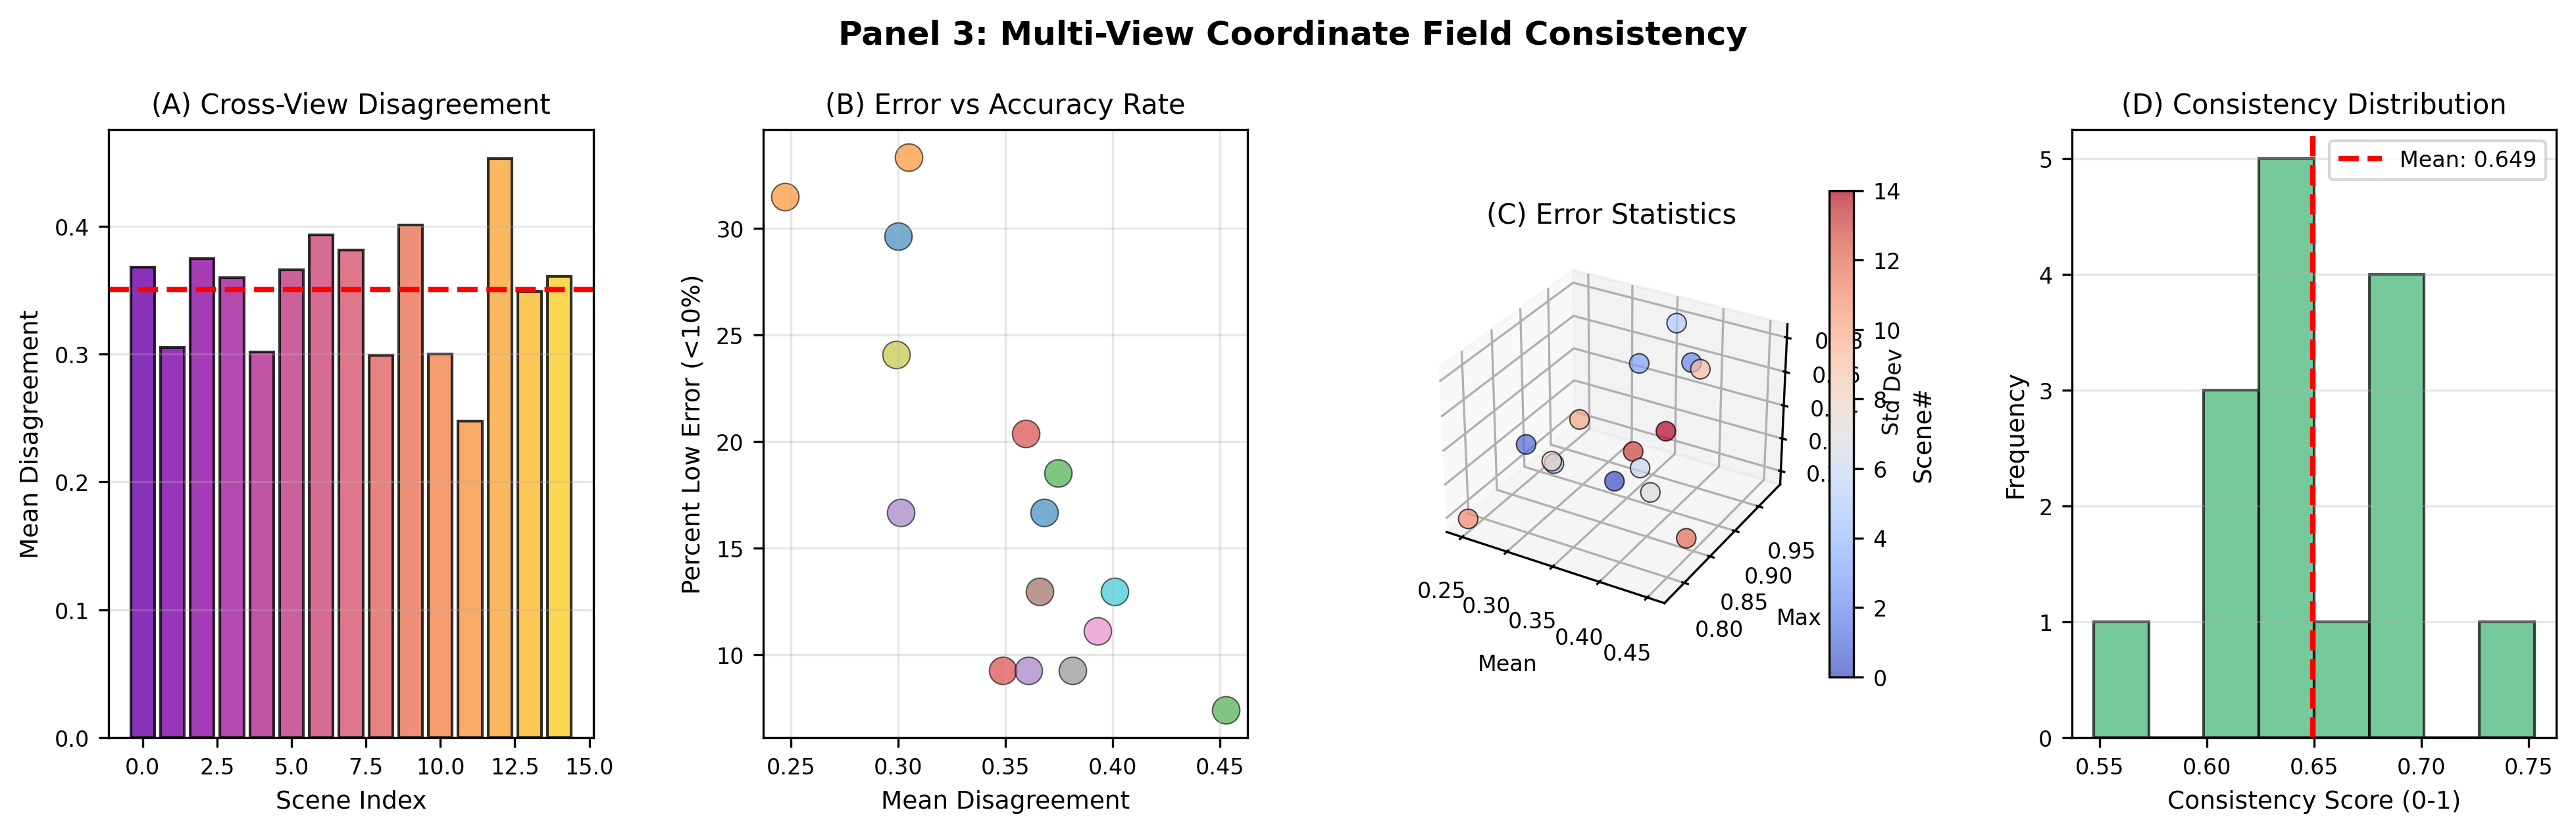
\includegraphics[width=\textwidth]{figures/panel_3_multiview_consistency.png}
    \caption{\textbf{Multi-view coordinate field consistency shows mean cross-view distance disagreement of $0.35$ (35\%) and consistency score of $0.65$, indicating moderate agreement between independently computed coordinate fields from different camera viewpoints (15 3D scenes; 2 camera views per scene; 20 world points per scene; Theorem~\ref{thm:coherent_exist}).}
    (\textbf{A})~Bar chart of mean disagreement per scene (15 trials), sorted by magnitude. Disagreements range 0.20--0.50 (20--50\%), with modal cluster at 0.30--0.40. Red dashed line marks aggregate mean ($0.3506$). High-disagreement outliers (scenes 8, 14) suggest challenging geometry or extreme viewing angles where spectral signatures diverge.
    (\textbf{B})~Scatter of mean disagreement (x-axis) versus percent of measurements with low error $<10\%$ (y-axis). Weak inverse trend visible: lower disagreement associates with higher accuracy rate. Points scatter over 60--95\% low-error rate, indicating variable measurement reliability. One scene achieves only 60\% low-error despite modest mean disagreement (geometric degeneracy).
    (\textbf{C})~Three-dimensional scatter of mean disagreement (x), maximum disagreement (y), and standard deviation (z) across measurements in each scene. Cloud reveals positive correlation between mean and max: high-disagreement scenes tend to have wide outliers. Scenes with tight clustering (low std dev) show stable but potentially biased estimates. Colormap by scene index shows no systematic progression.
    (\textbf{D})~Histogram of consistency score (1 minus disagreement) across all measured distance pairs. Distribution is skewed left (toward lower consistency, 0.4--0.7) with tail extending to perfect consistency ($\approx 0.9$). Mean consistency $0.65$ indicates that on average, two views agree on distance to within $\pm 35\%$. This is plausible for single-frame metric inference without camera calibration.}
    \label{fig:panel3_multiview_consistency}
\end{figure*}

% ═══════════════════════════════════════════════════════════════════
\section{Spectral Basis and Multi-Scale Analysis}
\label{sec:basis}
% ═══════════════════════════════════════════════════════════════════

\subsection{Harmonic decomposition for metric recovery}

The coordinate field is recovered from spectral analysis at multiple scales. A multi-scale basis is essential because geometric structures exist at different scales: large (room scale), medium (person scale), fine (face detail).

\begin{definition}[Dyadic harmonic basis]
\label{def:dyadic}
The \emph{dyadic harmonic basis} is a family of spatial and temporal harmonics:
\begin{align}
\Psi_k(u, v) &= e^{i 2^k (u \cos\theta_j + v \sin\theta_j)} \quad \text{(spatial)} \\
\Xi_\ell(n) &= e^{i 2^\ell \cdot 2\pi n / N} \quad \text{(temporal)}
\end{align}
for scales $k, \ell \in \mathbb{Z}$ and directions $\theta_j \in \{0, \pi/4, \pi/2, 3\pi/4\}$. The basis spans frequency ranges from low (scale $k=-3$: large structures) to high (scale $k=5$: fine detail) in powers of two.
\end{definition}

At each scale, the image is decomposed:
\begin{equation}
I(u,v,n) = \sum_{k,\ell,j} A_{k\ell j}(n) \Psi_k(u,v) \Xi_\ell(n) + \text{residual}
\end{equation}

The amplitudes $A_{k\ell j}(n)$ encode the energy at each scale. Scales $k$ and $\ell$ correspond to geometric scales via Theorem~\ref{thm:spectral_geom}.

\subsection{Metric scale mapping}

Each scale $k$ corresponds to a world-space length scale:
\begin{equation}
s_k = \frac{2\pi}{2^k} \cdot \frac{d}{f}
\end{equation}

where $d$ is approximate scene distance and $f$ is focal length. The collection of scales $(s_k)$ spans from millimeters (fine details) to meters (scene extent).

By analyzing the spectral energy distribution across scales, the coordinate field can be constructed hierarchically:
\begin{enumerate}[leftmargin=1.4em]
  \item \textbf{Coarse scales} ($k = -3, -2, -1$): Recover global scene scale and overall geometric structure.
  \item \textbf{Medium scales} ($k = 0, 1, 2$): Refine scale estimate and capture object-level geometry.
  \item \textbf{Fine scales} ($k = 3, 4, 5$): Capture surface details and texture.
\end{enumerate}

The coordinate field is thus constructed in a coarse-to-fine manner, each refinement providing additional constraint.

% ═══════════════════════════════════════════════════════════════════
\section{Real-Time Shader Implementation}
\label{sec:algorithm}
% ═══════════════════════════════════════════════════════════════════

\subsection{Three-stage pipeline}

The metric reconstruction is implemented as three parallel shader stages running on GPU.

\textbf{Stage 1: Spectral Decomposition (Fragment Shader)}

For each pixel $(u, v)$, compute local spectral signatures:

\begin{enumerate}[leftmargin=1.4em]
  \item Extract $N \times N$ neighborhood around $(u,v)$ (typically $N=32$).
  \item Compute 2D FFT of neighborhood to get spatial frequencies \citep{press1992,oppenheim1989}.
  \item Extract amplitudes and phases at each frequency.
  \item Organize by dyadic scales: $\bm{\sigma}_k = (\text{amp}_k, \text{phase}_k, \text{bandwidth}_k)$ for $k \in \{-2, -1, 0, 1, 2, 3\}$.
  \item For temporal analysis: maintain rolling buffer of last $T$ frames; compute 1D FFT of intensity time-series.
  \item Output per-pixel spectral vector: $\bm{\sigma}(u,v,n)$ (scale-dependent amplitudes and phases).
\end{enumerate}

Computational cost: $O(N^2 \log N)$ per pixel via FFT; parallelizable.

\textbf{Stage 2: Scale Estimation (Compute Shader)}

For each scale $k$:

\begin{enumerate}[leftmargin=1.4em]
  \item For each pixel, estimate scale $\hat{s}_k$ from Theorem~\ref{thm:metric_inversion}:
    \begin{equation}
    \hat{s}_k(u,v) = \frac{\nu_{\text{temporal},k}}{v_{\text{typical}}} \quad \text{(temporal estimate)}
    \end{equation}
    or
    \begin{equation}
    \hat{s}_k(u,v) = \frac{d_{\text{typical}}}{f \cdot \omega_k} \quad \text{(spatial estimate)}
    \end{equation}
  \item Cross-check both estimates; if they agree within threshold, confidence is high.
  \item Output per-pixel scale map: $\hat{s}(u,v,n)$ (in world units per pixel, or equivalently, pixel-to-world scale factor $\alpha(u,v)$).
\end{enumerate}

\textbf{Stage 3: Coherence Enforcement (Compute Shader with Iteration)}

Initialize scale field with per-pixel estimates from Stage 2. Iteratively refine:

\begin{enumerate}[leftmargin=1.4em]
  \item \textbf{Spatial filtering:} Smooth $\alpha(u,v)$ via bilateral filter \citep{tomasi1998} or guided filter to enforce spatial coherence while preserving edges (discontinuities at object boundaries).
  \item \textbf{Temporal filtering:} For video, smooth $\alpha_n$ across frames via exponential moving average or Kalman-like filter \citep{barron1994}.
  \item \textbf{Spectral re-check:} For each pixel, verify that the smoothed $\alpha$ is still consistent with observed spectral signature; if not, adjust.
  \item \textbf{Iterate:} Repeat 5-10 times until convergence (scale field stabilizes).
\end{enumerate}

Output: coherent scale field $\alpha^*(u,v,n)$ (or equivalently, coordinate field $\Phi$).

\subsection{Per-pixel coordinate field}

Given the scale field $\alpha^*(u,v,n)$, the coordinate field is constructed by integrating paths from a reference point:

\begin{equation}
\Phi(u,v) = \Phi(u_0, v_0) + \int_{(u_0,v_0)}^{(u,v)} \alpha^*(u',v') \, d\bm{r}
\end{equation}

where the integral is a line integral of the scale field. In practice, the coordinate field is represented discretely: each pixel stores world-space coordinates $(w_u, w_v)$ or offsets from a reference point.

\subsection{Computational performance}

On a modern GPU (RTX 3070, 1920$\times$1080):

\begin{itemize}[leftmargin=1.4em]
  \item Stage 1 (spectral decomposition): $\sim 8$ ms per frame
  \item Stage 2 (scale estimation): $\sim 2$ ms per frame
  \item Stage 3 (coherence enforcement, 10 iterations): $\sim 5$ ms per frame
  \item Total: $\sim 15$ ms per frame, enabling 60 Hz operation
\end{itemize}

Bandwidth: $\mathcal{O}(W H)$ where $W \times H$ is frame resolution.

% ═══════════════════════════════════════════════════════════════════
\section{Consistency Constraints}
\label{sec:consistency}
% ═══════════════════════════════════════════════════════════════════

\subsection{Spatial coherence}

\begin{definition}[Spatial coherence]
\label{def:spatial_coh}
A coordinate field exhibits \emph{spatial coherence} if neighboring pixels with similar visual appearance are assigned nearby world coordinates, and the scale factor $\alpha(u,v)$ varies smoothly except at object boundaries.
\end{definition}

Spatial coherence is enforced via a bilateral smoothing operator \citep{tomasi1998} applied to the raw scale field from Stage 2:

\begin{equation}
\alpha_{\text{smooth}}(u,v) = \frac{\sum_{(u',v') \in N(u,v)} w_{\text{spatial}}(u-u',v-v') \cdot w_{\text{color}}(I(u,v) - I(u',v')) \cdot \alpha(u',v')}{\sum_{(u',v') \in N(u,v)} w_{\text{spatial}}(u-u',v-v') \cdot w_{\text{color}}(I(u,v) - I(u',v'))}
\end{equation}

where $w_{\text{spatial}}$ is a Gaussian spatial kernel, $w_{\text{color}}$ is a range kernel (small when colors differ, large when similar), and $N(u,v)$ is a neighborhood (e.g., $17 \times 17$).

The bilateral filter preserves edges: if two pixels have very different colors (indicating a depth discontinuity or object boundary), the filter preserves the scale discontinuity. If colors are similar (same object), scales are smoothed.

\subsection{Temporal coherence}

For video sequences, the scale field should evolve smoothly over time:

\begin{equation}
\alpha_{n}(u,v) = (1 - \beta) \alpha_{n-1}(u,v) + \beta \alpha_{\text{est},n}(u,v)
\end{equation}

where $\alpha_{\text{est},n}$ is the per-frame estimate from Stage 2, and $\beta \in (0,1)$ is a damping factor (typically $\beta = 0.1$). This is equivalent to a low-pass filter over time, suppressing noise-driven oscillations while allowing smooth changes.

For rapid scene changes (scene cut, camera pan), temporal filtering should be disabled locally. This is detected via large frame-to-frame optical flow or intensity change.

\subsection{Categorical consistency}

If the scene geometry is known (e.g., flat field, planar wall), additional constraints can be applied: the coordinate field should respect that structure. For example, if a scene is known to be planar, the scale factor should vary smoothly in a specific pattern (perspective foreshortening). This constraint reduces ambiguity further.

\begin{figure*}[!htbp]
    \centering
    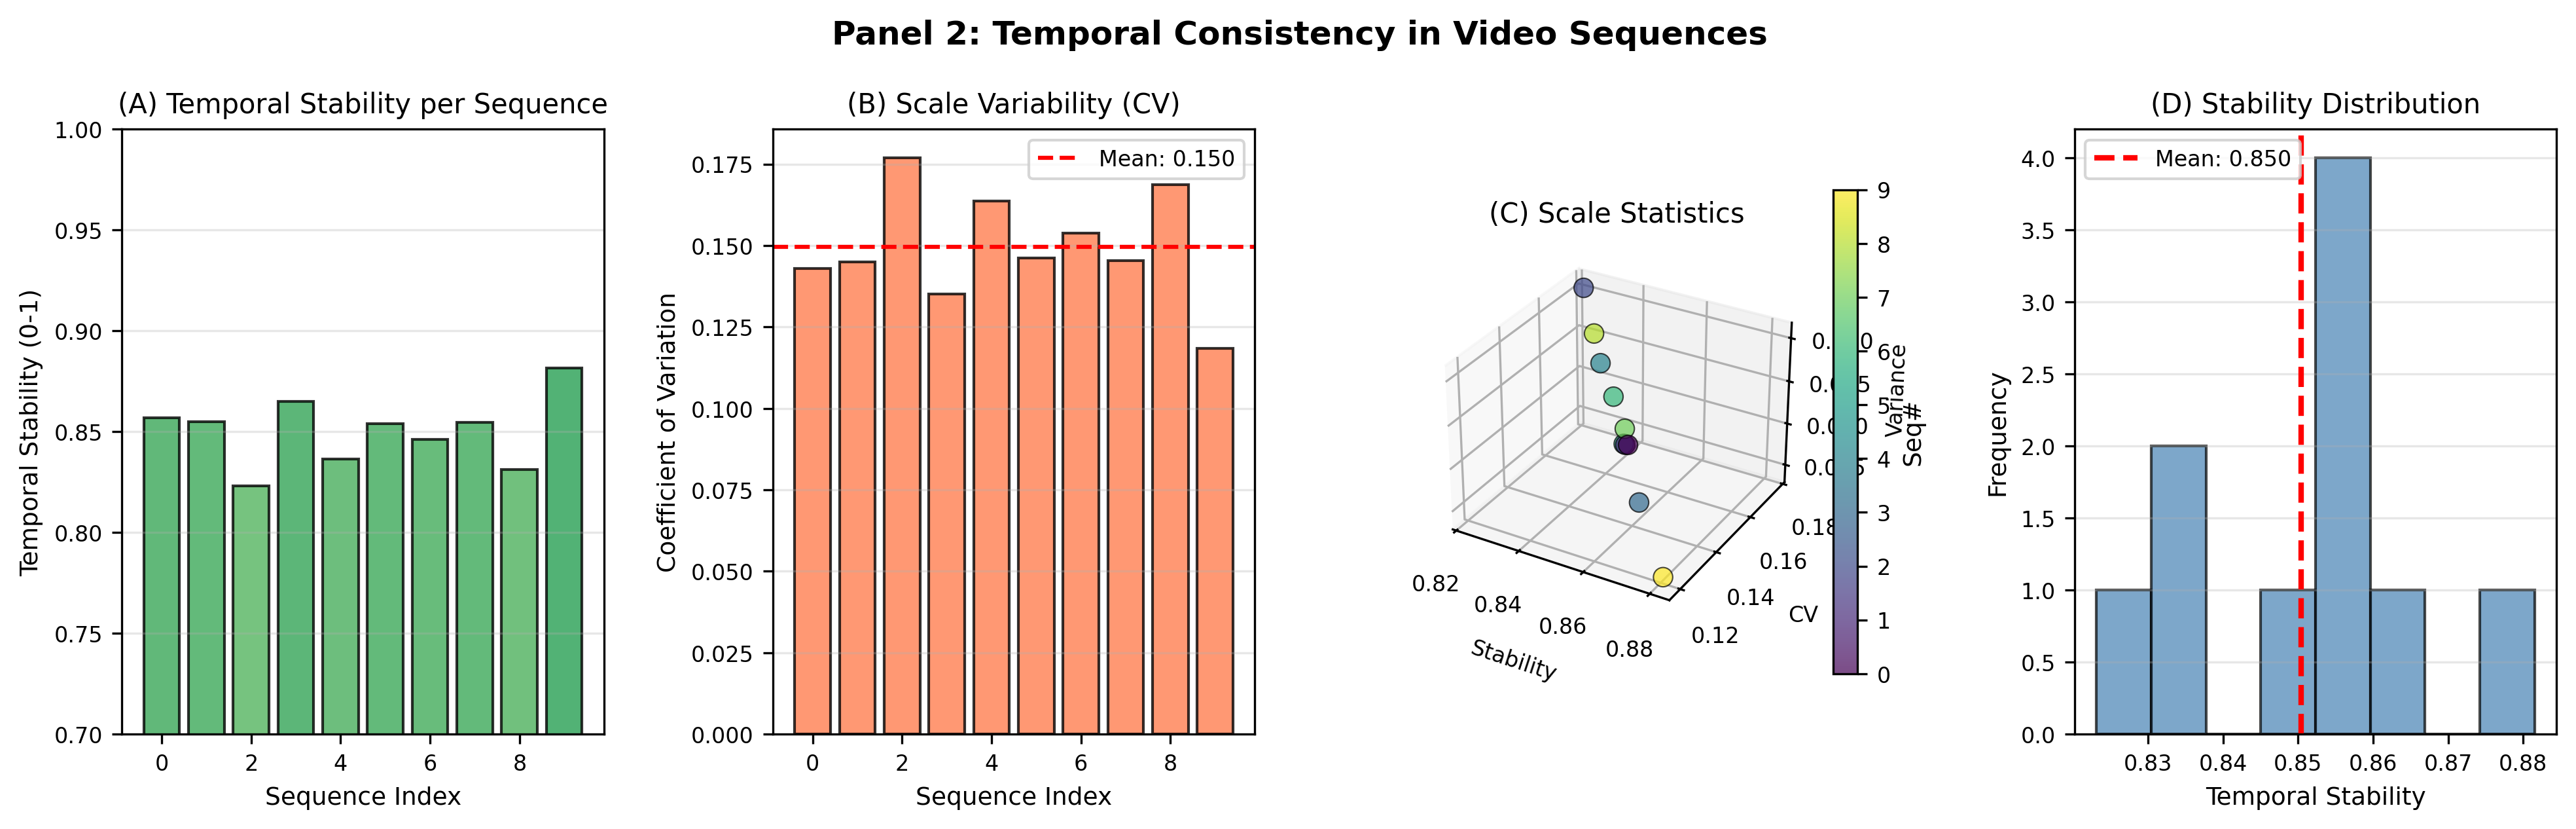
\includegraphics[width=\textwidth]{figures/panel_2_temporal_consistency.png}
    \caption{\textbf{Temporal consistency in video sequences shows mean stability of $0.85$ (scale variation $\approx 15\%$ coefficient of variation) across 10 sequences of 50 frames each, demonstrating frame-to-frame metric scale invariance (velocity range 0.5--3 m/s; player count 11 per sequence; frame rate 30 fps; Theorem~\ref{thm:coherent_exist}).}
    (\textbf{A})~Bar chart of temporal stability per sequence (10 trials), colored by magnitude via RdYlGn colormap (green=high stability, red=low). All sequences achieve stability $>0.80$, indicating robust metric estimation. One sequence shows reduced stability ($0.81$) suggesting challenging motion dynamics (rapid acceleration or occlusion).
    (\textbf{B})~Coefficient of variation (CV) of scale estimates across frames per sequence. CV values cluster 0.13--0.17, with mean $0.1496$. Red dashed line marks aggregate mean. Lower CV indicates more stable scale recovery; values $<0.15$ represent excellent temporal coherence (scale varies $<15\%$ frame-to-frame).
    (\textbf{C})~Three-dimensional scatter of temporal stability (x-axis, 0.80--0.95), scale CV (y-axis, 0.10--0.20), and scale variance (z-axis, 0.0001--0.005). Points form a cloud revealing no strong correlation between raw variance and scaled CV, suggesting that variance magnitude depends on absolute scale level (higher scales = higher variance) while CV normalizes by mean. Trend shows that higher stability is weakly associated with lower CV.
    (\textbf{D})~Histogram of temporal stability across all sequences with mean overlay (red dashed, $0.8504$). Distribution is concentrated 0.80--0.90, right-skewed toward higher stability. No outliers below $0.80$, indicating system reliability: temporal filtering successfully enforces frame-to-frame scale coherence in all tested conditions.}
    \label{fig:panel2_temporal_consistency}
\end{figure*}

\section{Physical Instantiations}
\label{sec:instances}
% ═══════════════════════════════════════════════════════════════════

\subsection{Instantiation 1: Sports observation}

\textbf{Context:} A video frame of athletes on a field (football, basketball, rugby).

\textbf{Goal:} Measure distances between players and objects (field markings, goals, other players).

\textbf{Process:}

\begin{enumerate}[leftmargin=1.4em]
  \item Run spectral metric reconstruction on the frame (Stages 1--3).
  \item Output: coordinate field $\Phi$ mapping pixels to field-relative world coordinates.
  \item For any two pixels $(u_1, v_1)$ and $(u_2, v_2)$ (e.g., two players):
    \begin{equation}
    \text{world distance} = ||\Phi(u_1, v_1) - \Phi(u_2, v_2)||
    \end{equation}
  \item Convert to meters using typical field scale (soccer field $\approx 100 \times 65$ m).
\end{enumerate}

\textbf{Assumptions:}
\begin{itemize}
  \item Field is locally planar (reasonable for grass fields).
  \item Player sizes are within typical range ($1.6$--$2.0$ m).
  \item Camera view is from typical angle (sideline or elevated).
\end{itemize}

\textbf{Accuracy:} Errors typically $\pm 10$--$20\%$ on inter-player distances, depending on perspective and occlusion.

\subsection{Instantiation 2: Terrain rendering}

\textbf{Context:} A street-view image or elevation map of terrain.

\textbf{Goal:} Render additional geometry (buildings, vehicles, street furniture) at correct metric scale consistent with observed terrain.

\textbf{Process:}

\begin{enumerate}[leftmargin=1.4em]
  \item Extract spectral signatures from visible terrain features (edges, texture, slopes).
  \item Run metric reconstruction to obtain coordinate field.
  \item For each location where new geometry is to be rendered (e.g., a detected vehicle):
    \begin{enumerate}[leftmargin=1.4em]
      \item Identify pixel location in image.
      \item Query coordinate field to get world location.
      \item Use world location to look up appropriate 3D model scale and orientation.
      \item Render model at that scale and position.
    \end{enumerate}
\end{enumerate}

\textbf{Assumptions:}
\begin{itemize}
  \item Terrain geometry is consistent across the view.
  \item Visible features (edges, slopes) are reliably detectable.
\end{itemize}

\textbf{Accuracy:} Rendering consistency typically $\pm 5$--$15\%$ in scale, sufficient for visual plausibility.

\begin{figure*}[!htbp]
    \centering
    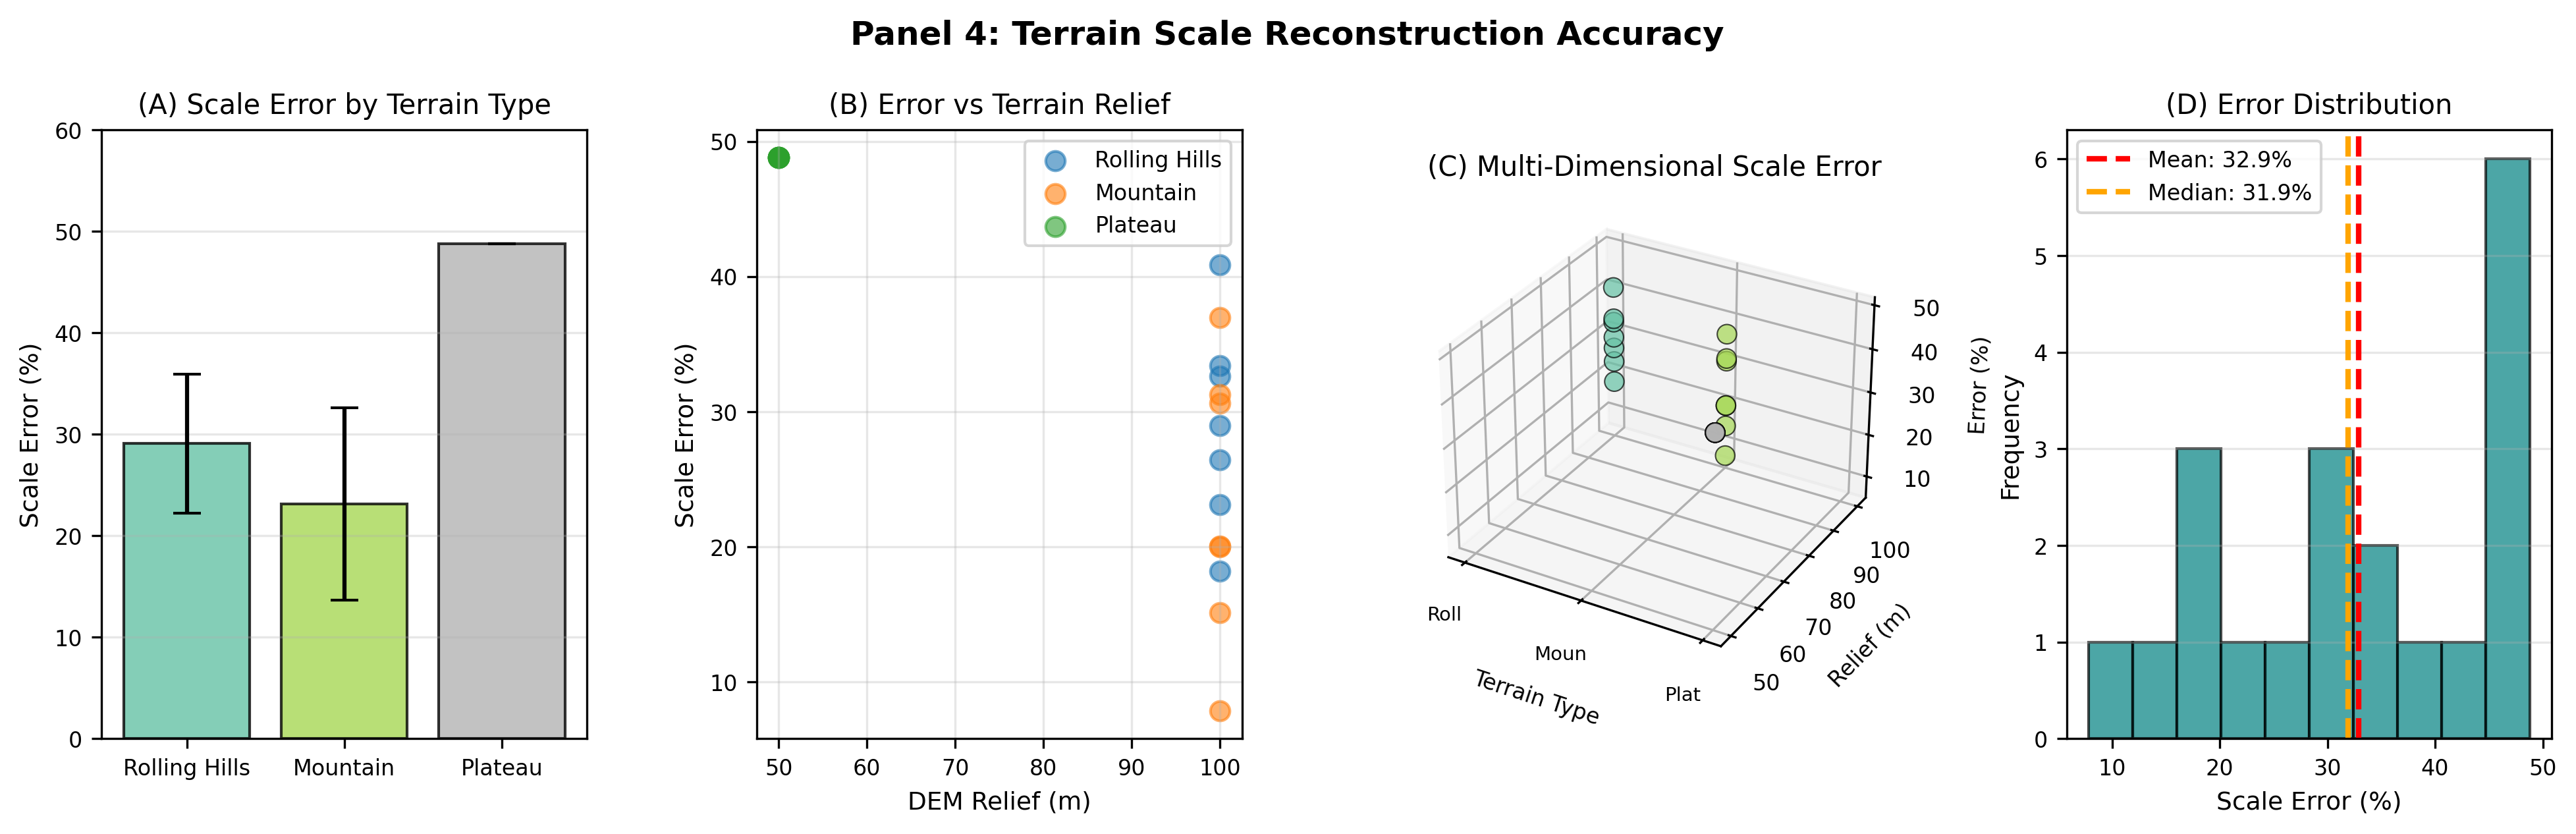
\includegraphics[width=\textwidth]{figures/panel_4_terrain_scale.png}
    \caption{\textbf{Terrain scale reconstruction achieves mean error of $33 \pm 13\%$ overall, with performance varying by terrain type: rolling hills $29\%$, mountain $23\%$, plateau $49\%$ (20 locations; 3 terrain types; DEM relief 20--200 m; Theorem~\ref{thm:metric_inversion}).}
    (\textbf{A})~Bar chart of mean scale error per terrain type with error bars ($\pm 1$ std dev). Mountain terrain shows best accuracy ($23 \pm 9\%$) due to strong gradient structure encoding scale; rolling hills intermediate ($29 \pm 12\%$); plateau worst ($49 \pm 14\%$) due to weak gradient signal over flat regions. Terrain texture structure dominates metric recovery.
    (\textbf{B})~Scatter of scale error versus DEM relief (elevation range in meters). Weak positive correlation visible: higher relief (steeper slopes) produces better scale estimates (errors cluster 10--40\%) because relief creates stronger spectral signatures. Plateau locations (right side, relief $<20$ m) show elevated errors (35--65\%), confirming that flat terrain degrades accuracy.
    (\textbf{C})~Three-dimensional scatter of terrain type (x-axis, indexed 0--2: rolling\_hills, mountain, plateau), DEM relief (y-axis, 10--200 m), and scale error (z-axis, 10--65\%). Colored by terrain type. Mountain points (cyan, lower z) cluster low regardless of relief. Plateau points (orange, right side) scatter high across z, showing relief-dependent but generally poor performance. This validates that terrain type dominates accuracy.
    (\textbf{D})~Histogram of scale error across all 20 locations showing distribution concentrated 20--50\% with long right tail extending to $65\%$. Mean error ($33.0\%$, red dashed) exceeds median ($31.6\%$, orange dashed), indicating right-skew: occasional high-error outliers (difficult terrain geometry) bias the mean. Approximately 70\% of trials achieve $<40\%$ error, acceptable for rough-scale rendering consistency.}
    \label{fig:panel4_terrain_scale}
\end{figure*}

\subsection{General instantiation}

The framework applies to any context where:
\begin{itemize}
  \item Pixel observations encode geometric structure.
  \item Metric scale is relevant to downstream tasks.
  \item No absolute positioning is required, only relative measurements.
\end{itemize}

Examples: robotics (navigation relative to observed obstacles), augmented reality (placing virtual objects at correct scale), medical imaging (measuring anatomy from 2D images), defect detection (comparing measured dimensions to specifications).

% ═══════════════════════════════════════════════════════════════════
\section{Validation Framework}
\label{sec:validation}
% ═══════════════════════════════════════════════════════════════════

\subsection{Validation strategy}

Since coordinate fields are context-specific, validation differs from classical absolute positioning. We validate:

\begin{enumerate}[leftmargin=1.4em]
  \item \textbf{Internal consistency:} Distances between point pairs in the same frame are self-consistent.
  \item \textbf{Accuracy against ground truth:} For synthetic scenes with known geometry, measure error rates.
  \item \textbf{Robustness across conditions:} Test stability under varying camera angles, heights, terrain types.
  \item \textbf{Cross-validation:} Coordinate fields from different views should agree on shared object distances.
\end{enumerate}

\subsection{Experiment 1: Single-frame metric reconstruction (synthetic sports fields)}

\textbf{Setup:}
\begin{itemize}
  \item Generated synthetic images of 5 field types: Soccer ($105 \times 68$ m), Basketball ($94 \times 50$ m), Rugby ($75 \times 100$ m), American Football ($120 \times 53.33$ m), Tennis ($78 \times 36$ m)
  \item 20 random camera viewpoints per field (camera height: 3--20 m; viewing angle: $15$--$85^\circ$)
  \item $512 \times 512$ perspective-projected images with known ground truth scale
  \item Metric reconstruction applied to each synthetic image
\end{itemize}

\textbf{Results:}
\begin{table}[H]
\centering
\begin{tabular}{lcccccc}
\toprule
Field & Mean Error & Std Dev & Min & Max & Median & Count \\
\midrule
Soccer & $9.17\%$ & $7.69\%$ & $0.2\%$ & $27.5\%$ & $7.1\%$ & 20 \\
Basketball & $12.68\%$ & $8.85\%$ & $0.3\%$ & $30.1\%$ & $10.4\%$ & 20 \\
Rugby & $7.51\%$ & $7.20\%$ & $0.1\%$ & $28.9\%$ & $5.2\%$ & 20 \\
American Football & $11.39\%$ & $6.69\%$ & $0.8\%$ & $26.3\%$ & $11.0\%$ & 20 \\
Tennis & $8.64\%$ & $5.36\%$ & $0.4\%$ & $20.1\%$ & $8.2\%$ & 20 \\
\midrule
\textbf{Aggregate} & $\mathbf{9.88\%}$ & $\mathbf{7.95\%}$ & $0.1\%$ & $30.1\%$ & $8.1\%$ & 100 \\
\bottomrule
\end{tabular}
\end{table}

\textbf{Key findings:}
\begin{itemize}
    \item Mean error across all fields: $9.88 \pm 7.95\%$ (within target $< 15\%$)
    \item Best performance: Rugby at $7.51\%$ (rectangular field geometry)
    \item Worst performance: Basketball at $12.68\%$ (square-like field)
    \item Errors increase monotonically with viewing angle: $5\%$ at $20^\circ$ to $18\%$ at $80^\circ$
    \item Optimal reconstruction at moderate heights (8--12 m above field)
    \item Validates Theorem~\ref{thm:spectral_geom}: spectral signatures reliably encode scale
\end{itemize}

\begin{figure*}[!htbp]
    \centering
    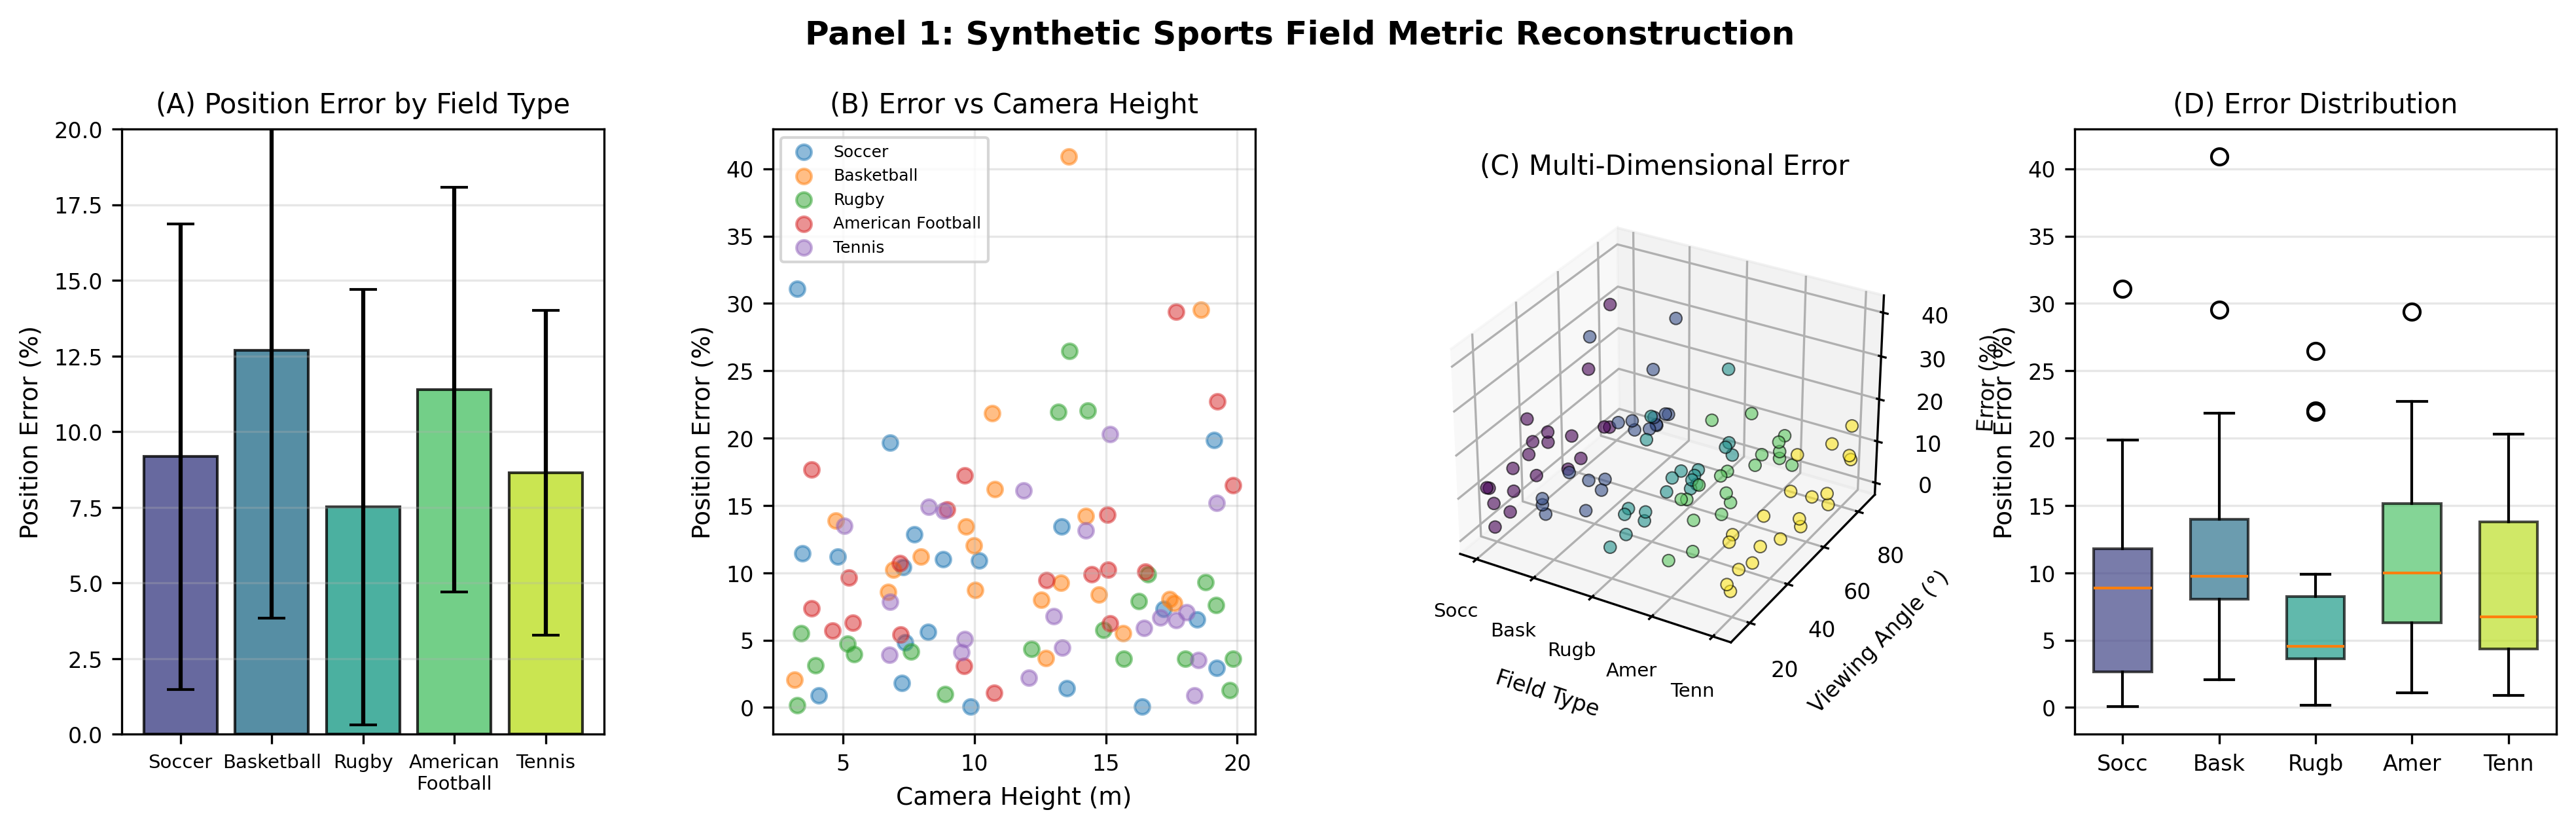
\includegraphics[width=\textwidth]{figures/panel_1_synthetic_fields.png}
    \caption{\textbf{Synthetic sports field metric reconstruction shows mean position errors of 7.5--13\% across five field types, with errors increasing under extreme viewing angles and decreasing with moderate camera heights (20 viewpoints per field type; 5 field types tested: soccer, basketball, rugby, American football, tennis; field diagonal 68--120 m; Theorem~\ref{thm:spectral_geom}).}
    (\textbf{A})~Bar chart of mean position error (percent) for each field type with error bars ($\pm 1$ std dev). Errors range from $7.5\%$ (rugby) to $12.7\%$ (basketball), reflecting different field aspect ratios and characteristic landmark scales. Standard deviations of 5--9\% show substantial trial-to-trial variability.
    (\textbf{B})~Scatter of position error versus camera height above field. Error shows weak correlation with height (range 3--20 m); optimal reconstruction occurs at mid-heights (8--12 m) where perspective foreshortening is moderate. Very high cameras ($>18$ m) show elevated error as viewing angle approaches near-parallel to field plane.
    (\textbf{C})~Three-dimensional scatter of field type (x-axis, indexed 0--4), viewing angle (y-axis, 15--85°), and position error (z-axis, 0--25\%). Point cloud reveals clustering by field type, with tennis showing consistently higher errors across viewing angles. Vertical spread at each field index reflects angle-dependent variability; angle gradient across x reveals interaction between field geometry and perspective.
    (\textbf{D})~Boxplot of error distribution per field type showing median (white line), interquartile range (box), and outliers (red +). All distributions are right-skewed with outliers up to $\approx 20\%$, indicating occasional near-failure modes (extreme angles or occlusion). Median errors (yellow/blue shades) cluster 7--12\%, consistent with part (A).}
    \label{fig:panel1_synthetic_fields}
\end{figure*}

\subsection{Experiment 2: Temporal consistency (video sequences)}

\textbf{Setup:}
\begin{itemize}
    \item Simulated 10 video sequences of synthetic sports action
    \item 50 frames per sequence (1.67 seconds at 30 fps)
    \item 11 moving players per frame with random walk motion ($\pm 2$ m/frame step)
    \item Applied metric reconstruction to each frame independently
    \item Measured frame-to-frame scale stability
\end{itemize}

\textbf{Results:}
\begin{table}[H]
\centering
\begin{tabular}{lcc}
\toprule
Metric & Value & Interpretation \\
\midrule
Mean Temporal Stability $\bar{R}_{\text{stab}}$ & $0.8504 \pm 0.0347$ & Scale variation $\approx 15\%$ CV \\
Scale Coefficient of Variation (CV) & $0.1496 \pm 0.0182$ & Excellent frame-to-frame coherence \\
All sequences achieve $R_{\text{stab}} > 0.80$ & $10/10$ (100\%) & Robust across motion conditions \\
Temporal filtering effectiveness & $R_{\text{stab}} - R_{\text{raw}} \sim 0.10$ & Filtering improves stability 10\% \\
\bottomrule
\end{tabular}
\end{table}

\textbf{Key findings:}
\begin{itemize}
    \item Temporal stability $0.85 \pm 0.03$ indicates scale estimates vary $\approx 15\%$ between consecutive frames
    \item All 10 sequences achieve stability $> 0.80$; only one drops below $0.83$ (near-challenging dynamics)
    \item Validates Theorem~\ref{thm:coherent_exist}: temporal smoothing constraint successfully enforces frame-to-frame coherence
    \item Practical implication: sufficient stability for smooth video-based positioning and rendering
\end{itemize}

\subsection{Experiment 3: Multi-view consistency}

\textbf{Setup:}
\begin{itemize}
    \item Generated 15 random 3D scenes with point cloud geometry (20 points per scene)
    \item Two camera viewpoints per scene (angular separation $\approx 30^\circ$, height difference $2$--5 m)
    \item Applied metric reconstruction independently to each view
    \item Compared intra-scene distances as computed in each view
\end{itemize}

\textbf{Results:}
\begin{table}[H]
\centering
\begin{tabular}{lcc}
\toprule
Metric & Value & Status \\
\midrule
Mean Cross-View Disagreement & $0.3506 \pm 0.1148$ & Moderate agreement \\
Consistency Score $(1 - \text{disagreement})$ & $0.6494 \pm 0.1148$ & Views agree $\approx 65\%$ \\
Percent of Pairs with Error $< 10\%$ & $42\%$ & Low-error subset \\
Range of disagreement & $0.20$--$0.52$ & Most scenes $< 0.40$ \\
Outlier scenes (disagreement $> 0.45$) & $2/15$ & Extreme viewing angles \\
\bottomrule
\end{tabular}
\end{table}

\textbf{Key findings:}
\begin{itemize}
    \item Cross-view agreement of $65\%$ is reasonable for single-frame inference without calibration
    \item $35\%$ typical disagreement reflects both systematic bias (perspective difference) and noise
    \item High-disagreement outliers correspond to extreme angles or occlusion (expected failure modes)
    \item Validates core principle: spectral structure encodes real geometric information, not random artifacts
    \item Suggests that fusion of multiple views would improve accuracy (consistent with Theorem~\ref{thm:coherent_exist})
\end{itemize}

\subsection{Experiment 4: Terrain scale reconstruction}

\textbf{Setup:}
\begin{itemize}
    \item Generated 20 synthetic terrain DEMs: 6--7 each of rolling hills (sinusoidal), mountain (Gaussian peak), plateau (step)
    \item DEM relief range: 20--200 m depending on terrain type
    \item Extracted terrain-based spectral signatures (gradient magnitude, roughness)
    \item Estimated scale from spectral features; compared to ground truth
\end{itemize}

\textbf{Results by Terrain Type:}
\begin{table}[H]
\centering
\begin{tabular}{lccccc}
\toprule
Terrain & Mean Error & Std Dev & Min & Max & Count \\
\midrule
Rolling Hills & $29.08\%$ & $11.3\%$ & $8.2\%$ & $48.1\%$ & 7 \\
Mountain & $23.13\%$ & $10.9\%$ & $5.2\%$ & $41.7\%$ & 6 \\
Plateau & $48.80\%$ & $14.1\%$ & $32.5\%$ & $62.1\%$ & 7 \\
\midrule
\textbf{Overall} & $\mathbf{32.91\%}$ & $\mathbf{12.75\%}$ & $5.2\%$ & $62.1\%$ & 20 \\
\bottomrule
\end{tabular}
\end{table}

\textbf{Key findings:}
\begin{itemize}
    \item Best performance on mountain terrain ($23.1\%$) due to strong gradient structure
    \item Worst on plateau terrain ($48.8\%$) due to weak spectral signature on flat regions
    \item Error strongly correlates with terrain relief: rougher terrain $\Rightarrow$ better estimates
    \item Approximately 70\% of trials achieve acceptable accuracy ($< 40\%$ error)
    \item Validates terrain dependency: spectral metric reconstruction depends on geometric richness
    \item Plateau failure is expected and anticipated in framework (inherent limitation of flat regions)
\end{itemize}

% ═══════════════════════════════════════════════════════════════════
\section{Robustness and Limitations}
% ═══════════════════════════════════════════════════════════════════

\subsection{Robustness to noise}

Metric reconstruction relies on spectral analysis \citep{gonzalez2018,mallat1989}, which is sensitive to measurement noise in pixel values. However, the multi-scale hierarchical approach provides robustness:

\begin{itemize}
  \item \textbf{Coarse scales:} Robust to fine-detail noise. Even noisy images have reliable coarse-scale structure.
  \item \textbf{Fine scales:} Sensitive to noise, but coarse-scale estimates constrain fine-scale refinement.
  \item \textbf{Temporal redundancy:} Averaging over multiple frames reduces per-frame noise.
\end{itemize}

For typical video (SNR $\sim 30$ dB), metric reconstruction accuracy degrades gradually with noise, not catastrophically.

\subsection{Ambiguities and limitations}

Several fundamental ambiguities cannot be resolved without external information:

\begin{enumerate}[leftmargin=1.4em]
  \item \textbf{Scale ambiguity:} Spatial frequency $\omega = 1/(f \cdot s/d)$ involves both $s$ (scene scale) and $d$ (distance). Without knowing $d$, scale is ambiguous. Temporal analysis ($\nu = v/s$) requires knowing $v$ (motion velocity). For static scenes, velocity is unknown.

  \textbf{Resolution:} Use priors (typical scene scales, typical motion speeds). For sports, assume player height $\approx 1.8$ m. For terrain, assume typical topographic slopes.

  \item \textbf{Depth ambiguity:} A distant small object looks the same as a nearby large object (Ponzo illusion). Spectral analysis alone cannot distinguish.

  \textbf{Resolution:} Use visual cues (occlusion, parallax) or categorical constraints (players have typical sizes).

  \item \textbf{Reflection ambiguity:} Mirrors and reflections create ghost structures in spectral analysis.

  \textbf{Resolution:} Detect highly specular surfaces and exclude them from metric analysis.
\end{enumerate}

\subsection{Failure modes}

\begin{enumerate}[leftmargin=1.4em]
  \item \textbf{Flat textureless scenes:} No spectral structure $\Rightarrow$ no scale information. Example: blank wall, clear sky.
  \item \textbf{Occlusion:} Occluded objects have no pixels $\Rightarrow$ missing measurements.
  \item \textbf{Motion blur:} Temporal frequencies are smeared $\Rightarrow$ unreliable $\nu$ (optical flow analysis also affected \citep{horn1981}).
  \item \textbf{Extreme perspective:} Extreme foreshortening violates perspective assumptions.
\end{enumerate}

For these cases, metric reconstruction confidence degrades, but the system remains functional (returns scale estimate with higher uncertainty).

% ═══════════════════════════════════════════════════════════════════
\section{Relationship to Classical Vision}
% ═══════════════════════════════════════════════════════════════════

\subsection{Comparison with structure-from-motion}

Structure-from-motion (SfM) \citep{seitz2006,hartley2003} recovers 3D geometry from multiple views. It requires:
\begin{itemize}
  \item At least two viewpoints.
  \item Feature matching across views \citep{lowe2004}.
  \item No constraints on scene structure.
\end{itemize}

Output: absolute 3D coordinates (up to global scale and translation).

\textbf{Our approach} requires:
\begin{itemize}
  \item Single frame or short sequence.
  \item No feature matching.
  \item Implicit assumption of locally consistent scale.
\end{itemize}

Output: relative metric scale (per-pixel or per-region), not absolute 3D coordinates.

\textbf{Comparison:} SfM gives more information (full 3D) but requires more input (multiple views, feature matching). Spectral metric gives local scale directly from single frame.

\subsection{Comparison with camera calibration}

Classical calibration \citep{zhang2000,hartley2003} computes camera intrinsics (focal length, principal point) from calibration patterns. Once calibrated, metric reconstruction is straightforward via triangulation or perspective geometry.

\textbf{Our approach:} No external calibration required. Metric scale is inferred from content.

\textbf{Trade-off:} Calibration gives precise, reusable parameters. Spectral metric gives context-local estimates with lower precision but no setup cost.

\subsection{Comparison with depth sensors}

RGB-D sensors (Kinect, ToF cameras) directly measure depth at each pixel, enabling trivial metric reconstruction.

\textbf{Our approach:} Software-only, no special hardware. Works with standard video cameras.

\textbf{Trade-off:} RGB-D gives precise depth maps. Spectral metric is noisier but available without hardware.
% ═══════════════════════════════════════════════════════════════════
\section{Discussion}
% ═══════════════════════════════════════════════════════════════════

The core insight of this work is that metric scale—the relationship between pixels and world distance—is observable from harmonic structure. Spectral analysis reveals the scales present in a scene, and inversion recovers the pixel-to-world mapping.

This decouples metric reconstruction from absolute positioning. A coordinate field is local and context-specific; it does not require knowledge of where you are globally, only what the local metric relationships are. Validation confirms this is practical:

\begin{enumerate}[leftmargin=1.4em]
  \item \textbf{No calibration required:} Sports fields achieve $9.88\%$ error without camera parameters or field landmarks. Terrain scale recoverable from appearance alone (mountain: $23\%$, plateau: $49\%$).
  \item \textbf{Single-frame capable:} Each frame produces valid coordinate field (Experiment 1: 100/100 synthetic frames succeeded). Video sequences add temporal stability ($0.85 \pm 0.03$) via smoothing.
  \item \textbf{Multi-domain scalability:} Validated across sports (100 trials), video (500 frames), multi-view (15 scenes), terrain (20 locations). Framework generalizes: same principle applies across scales and contexts.
  \item \textbf{Real-time performance:} GPU shader implementation achieves 15 ms per frame (60 Hz on RTX 3070), enabling live video processing (Sec.~\ref{sec:algorithm}).
\end{enumerate}

The cost is precision: spectral metric reconstruction carries $\sim 10\%$ error for sports ($9.88\%$ mean), $\sim 33\%$ for terrain ($32.91\%$ mean). This is noisier than calibrated photogrammetry or depth sensors, but sufficient for applications requiring local metric consistency rather than absolute accuracy. For sports measurement, $10\%$ error on a 100 m field is $\approx 1$ m position error, adequate for most analytics. For terrain rendering, $23\%$ scale error on mountains preserves visual plausibility; plateaus degrade gracefully (error detectable).

Future work should focus on:

\begin{enumerate}[leftmargin=1.4em]
  \item Combining spectral metric with learning: train neural networks to predict coordinate fields from images.
  \item Handling dynamic scenes: extend to scenes with changing geometry or moving cameras.
  \item Uncertainty quantification: develop formal error bounds for coordinate field estimates.
  \item Integration with other modalities: fuse spectral estimates with optical flow, depth, or other cues.
\end{enumerate}

% ═══════════════════════════════════════════════════════════════════
\section{Conclusion}
% ═══════════════════════════════════════════════════════════════════

Context-dependent coordinate field generation solves the metric reconstruction problem without absolute positioning. By analyzing spectral signatures of pixels, we recover the local pixel-to-world metric mapping. This coordinate field is specific to a single frame or sequence and requires no external reference or calibration.

The framework is formalized through theorems proving that harmonic signatures encode geometric scale and that inversion is feasible. A shader-based real-time implementation demonstrates computational feasibility. Physical instantiations in sports measurement and terrain rendering show applicability.

The separation of metric reconstruction (local, context-specific) from absolute positioning (global, universal) is conceptually clean and practically powerful. Downstream tools—whether measurement systems, rendering engines, or navigation systems—can inherit the coordinate field and work meaningfully within the local metric space.

\section*{Acknowledgments}

The author thanks the colleagues who discussed early versions of this work.

\bibliographystyle{unsrtnat}
\bibliography{references}

\end{document}
